%% @Author: Ines Abdeljaoued Tej
%  @Date:   2018-02
%% @Class:  Posters pour l'ESSAI - Universite de Carthage, Tunisie.

%%%%%%%%%%%%%%%%%%%%%%%%%%%%%%%%%%%%%%%%%
% a0poster Portrait Poster
% LaTeX Template
% Version 1.0 (22/06/13)
%
% The a0poster class was created by:
% Gerlinde Kettl and Matthias Weiser (tex@kettl.de)
%
% This template has been downloaded from:
% http://www.LaTeXTemplates.com
%
% License:
% CC BY-NC-SA 3.0 (http://creativecommons.org/licenses/by-nc-sa/3.0/)
%
%%%%%%%%%%%%%%%%%%%%%%%%%%%%%%%%%%%%%%%%%

%----------------------------------------------------------------------------------------
%	PACKAGES AND OTHER DOCUMENT CONFIGURATIONS
%----------------------------------------------------------------------------------------

\documentclass[a0, portrait]{a0poster}
\usepackage[top=5cm, bottom=0.3cm, left=5cm, right=3cm]{geometry}
\usepackage[compact]{titlesec}
\usepackage{multicol}

\usepackage[frenchb]{babel}
\usepackage{ifxetex}
\ifxetex
  \usepackage{fontspec}
\else
  \usepackage[T1]{fontenc}
  \usepackage[utf8]{inputenc}
  \usepackage{lmodern}
\fi


\usepackage{multicol} % This is so we can have multiple columns of text side-by-side
\columnsep=100pt % This is the amount of white space between the columns in the poster
\columnseprule=3pt % This is the thickness of the black line between the columns in the poster

\usepackage[svgnames]{xcolor} % Specify colors by their 'svgnames', for a full list of all colors available see here: http://www.latextemplates.com/svgnames-colors

\usepackage{times} % Use the times font
%\usepackage{palatino} % Uncomment to use the Palatino font

\usepackage{graphicx} % Required for including images
\graphicspath{{figures/}} % Location of the graphics files
\usepackage{booktabs} % Top and bottom rules for table
\usepackage[font=small,labelfont=bf]{caption} % Required for specifying captions to tables and figures
\usepackage{amsfonts, amsmath, amsthm, amssymb} % For math fonts, symbols and environments
\usepackage{wrapfig} % Allows wrapping text around tables and figures

\begin{document}

%----------------------------------------------------------------------------------------
%	POSTER HEADER
%----------------------------------------------------------------------------------------

% The header is divided into two boxes:
% The first is 75% wide and houses the title, subtitle, names, university/organization and contact information
% The second is 25% wide and houses a logo for your university/organization or a photo of you
% The widths of these boxes can be easily edited to accommodate your content as you see fit

\begin{minipage}[b]{0.75\linewidth}
\VeryHuge \color{NavyBlue} \textbf{Les problèmes avec les écoles en l'Afrique} \color{Black}\\[0.5cm]% Title
\Huge\textit{Une étude sur les problèmes }\\[0.5cm]% Subtitle
\end{minipage}
%
\begin{minipage}[b]{0.25\linewidth}

\includegraphics[width=7cm]{logo-essai.jpg}
\end{minipage}

\begin{minipage}[b]{0.75\linewidth}
\huge \textbf{Hamza BELHADJ AHMED}\\[0.5cm] % Author(s)
\Large Ecole Sup\'erieure de la Statistique et de l'Analyse de l'Information, Université de Carthage, Tunisie\\[0.4cm] % University/organization
\large \texttt{hmzblhdjahmd@gmail.com}\\
\end{minipage}


\vspace{1cm} % A bit of extra whitespace between the header and poster content

%----------------------------------------------------------------------------------------

\begin{multicols}{3} % This is how many columns your poster will be broken into, a portrait poster is generally split into 2 columns

%----------------------------------------------------------------------------------------
%	ABSTRACT
%----------------------------------------------------------------------------------------

\color{Navy} % Navy color for the abstract

\begin{abstract}
On va étudier et analyser les différents problèmes avec les écoles que les pays de l'Afrique possèdent.
\end{abstract}
%----------------------------------------------------------------------------------------
%	INTRODUCTION
%----------------------------------------------------------------------------------------

\color{Black} % SaddleBrown color for the introduction
\section*{Introduction}

\begin{itemize}
\item Rorem ipsum dolor sit amet, consectetur adipisicing elit.

\item From sunt in culpa qui officia deserunt mollit anim id est laborum.
\end{itemize}
%----------------------------------------------------------------------------------------
%	GEOLOGY
%----------------------------------------------------------------------------------------

\color{Black} % DarkSlateGray color for the rest of the content

\section*{Thématique choisie}
The geology of Algeria (Figure 1) is divided into two main structural units: the folded Tellian Domain in the North, and the Saharian Platform in the South, separated by the South Atlasic Flexure (Fabre, 1976).
\begin{center}\vspace{1cm}
% \includegraphics[width=0.8\linewidth]{Figure_1}
% \captionof{figure}{\color{Green} Major geotectonics units of West Africa modified from Fabre (1976). 1: Tertiary and Quaternary; 2: Alpine molasses; 3: Tertiary thrust sheet; 4: Secondary tabular; 5: Secondary plicative; 6: Primary plicative; 7: Primary tabular; 8: Precambrian and Precorce Cambrian of Sahara; 9: Cenozoic magma; 10: Megafault.}
\end{center}%\vspace{1cm}
%----------------------------------------------------------------------------------------
%	GEOTHERMAL DATA
%----------------------------------------------------------------------------------------
\section*{Description des données}
\subsection*{Heat Flow}
\begin{itemize}
\item Average heat flow values are 82$\pm19$ mW/m$^2$
\item Very high heat flow values (90-130 mW/m$^2$) in South Algeria (Hoggar Precambrian basement).
\end{itemize}
\begin{center}\vspace{1cm}
%\includegraphics[width=1.0\linewidth]{Fig2}
%\captionof{figure}{\color{Green} (A) Temp. vs. depth for different regions (Takherist and Lesquer, 1989). (B) Heat flow map of Algeria (Takherist and Lesquer, 1989). Unit: mW/m$^2$. 230 oil wells are presented, with depths ranging from 500 to 5500 m.}
\end{center}\vspace{1cm}

%------------------------------------------------

\begin{center}\vspace{1cm}
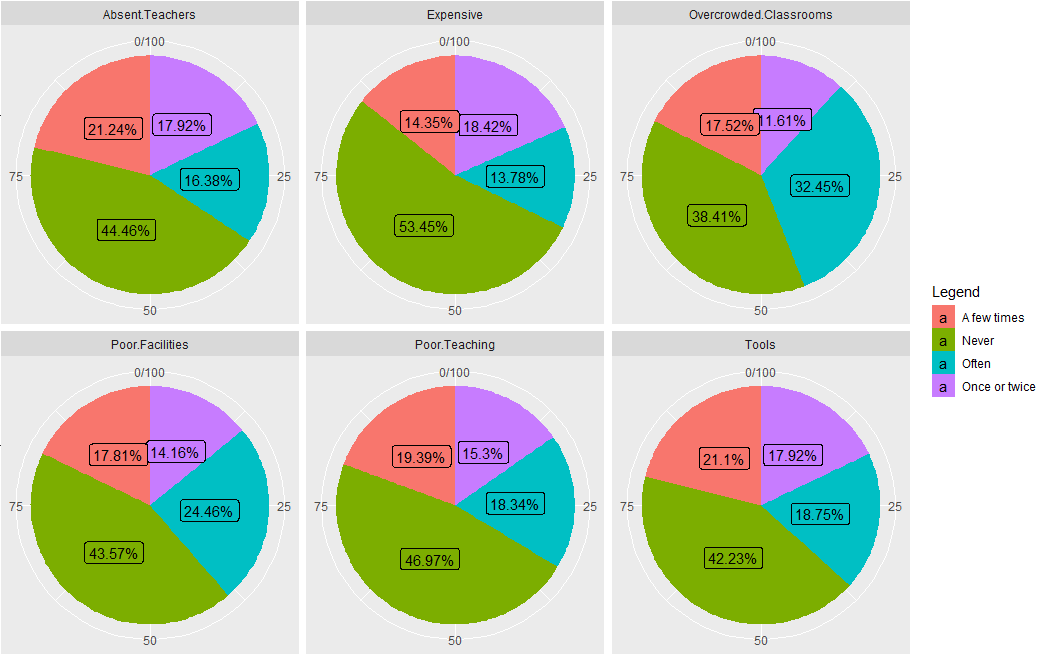
\includegraphics[width=0.8\linewidth]{fig_6_pie.png}
\captionof{figure}{\color{Green} Main Algerian geothermal areas (Fekraoui and Abouriche, 1995)}
\end{center}\vspace{1cm}

\begin{center}\vspace{1cm}
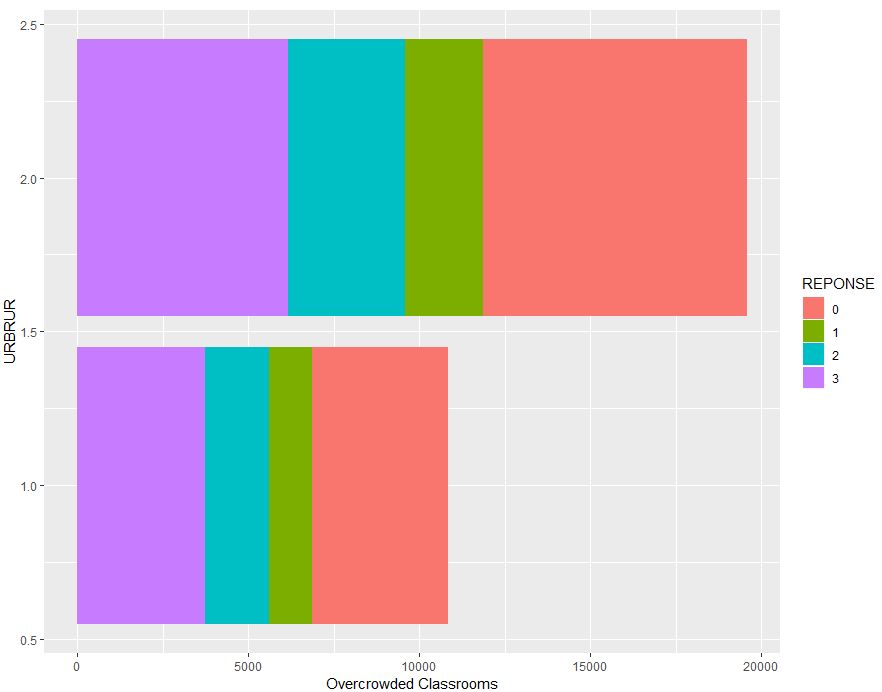
\includegraphics[width=0.8\linewidth]{fig_classrooms_urbrur.png}
\captionof{figure}{\color{Green} Temperatures of the main hot springs of the northern part of Algeria (Kedaid, 2002)}
\end{center}\vspace{1cm}

%----------------------------------------------------------------------------------------
%	CONCLUSIONS
%----------------------------------------------------------------------------------------

\color{SaddleBrown} % SaddleBrown color for the conclusions to make them stand out

\section*{Conclusions}

Tempor incididunt ut labore et dolore magna aliqua. Ut enim ad minim veniam,
quis nostrud exercitation ullamco laboris nisi ut aliquip ex ea commodo
consequat. Duis aute irure dolor in reprehenderit in voluptate velit esse
cillum dolore eu fugiat nulla pariatur. Excepteur sint occaecat cupidatat non
proident, sunt in culpa qui officia deserunt mollit anim id est laborum. Lorem ipsum dolor sit amet, consectetur adipisicing elit, sed do eiusmod
tempor incididunt ut labore et dolore magna aliqua. Ut enim ad minim veniam,
quis nostrud exercitation ullamco laboris nisi ut aliquip ex ea commodo
consequat.

\color{Black} % Set the color back to DarkSlateGray for the rest of the content

%----------------------------------------------------------------------------------------
%	FORTHCOMING RESEARCH
%----------------------------------------------------------------------------------------

\section*{Perspectives}

Quis nostrud exercitation ullamco laboris nisi ut aliquip ex ea commodo
consequat. Duis aute irure dolor in reprehenderit in voluptate velit esse
cillum dolore eu fugiat nulla pariatur. Excepteur sint occaecat cupidatat non
proident, sunt in culpa qui officia deserunt mollit anim id est laborum \cite{ggmap,mapdata}.


 %----------------------------------------------------------------------------------------
%	REFERENCES
%----------------------------------------------------------------------------------------

\nocite{*} % Print all references regardless of whether they were cited in the poster or not
\bibliographystyle{plain} % Plain referencing style
\bibliography{sample} % Use the example bibliography file sample.bib

%----------------------------------------------------------------------------------------

\end{multicols}
\end{document}